\begin{comment}
Dette må endres, for dette er feil! 
\end{comment}

\subsection{Representing the Underlying Structure}
It is important that the category names are identical at all places they occur. Wikipedia is written by volunteers from all over the worlds, and users might use different encoding depending on where they are from. Thus, both a cleaning process and a normalization process should be performed on all category names. The cleaning process is to make the category names look readable, while the normalization is a process where all words are made equal regardless of character encoding \cite[p.~26]{iirbook}.

Figure \ref{fig:withnewline} is an example of a \texttt{INSERT} statement which represents a link between the category \emph{fictional\_birds} and the subcategory \emph{ducks\textbackslash n fictional ducks}. This statement is an example of two category names that need to be processed so that they appear as \emph{ficitonal birds} and \emph{fictional ducks}. This processing  is usually called a \emph{data cleaning process} \cite{datacleaning}. The data cleaning for our purpose is converting all words to lowercase, replacing underscores with spaces and splitting up titles containing the code for newline (\emph{\textbackslash n}). Wikipedia uses the code for newline to represent how the articles should be sorted. Figure \ref{fig:fictionalbirds} shows that \emph{fictional ducks} are sorted as if it started with the word \emph{ducks}.

%The cleaning process includes converting all words to lowercase, replacing underscores with spaces and splitting up all titles containing the code for newline (\emph{\textbackslash n}). Newline is a way of representing how the articles should be sorted, figure \ref{fig:withnewline} is an example of an \texttt{INSERT} statement with newline in the title of the category, where the category should be sorted as if the title was \emph{ducks} as seen in figure \ref{fig:fictionalbirds}. Hence, the relevant part of the category title is the part after the newline, and this is the part that is considered further in the results. 
% Write something about normalization here. 

%Newline inside a category title is a way for Wikipedia to save space about the category nformation.  An example of such a statement is found in figure \ref{fig:withnewline}. 

%\footnote{TODO: insert reference: part of the insertion statement from the file \enwikicatlink} 

\begin{figure}[h]
\begin{lstlisting}
(1517681,'fictional_birds','ducks\nfictional ducks','2014-10-26 03:30:11',
'ducks','uppercase','subcat')
\end{lstlisting}
\caption[\texttt{INSERT} statement with newline]{Excerpt from \texttt{enwiki-latest-categorylinks.sql.gz} showing an \texttt{INSERT} statement including a newline character. }
\label{fig:withnewline}
\end{figure}

\begin{figure}[h]
\centering
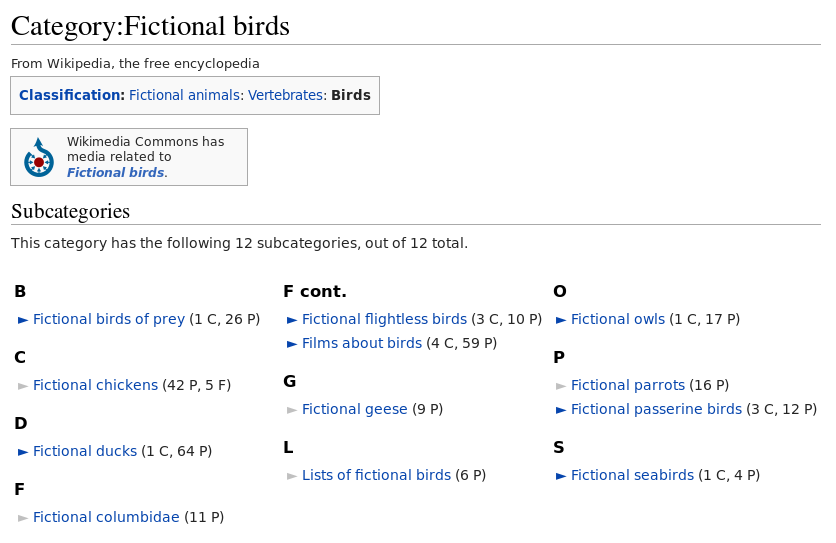
\includegraphics[width=\textwidth]{Chapters/Implementation/Fictional_birds_2}
\caption{The subcategories of the category \emph{Fictional birds} and how its subcategories are sorted based on the defined sortkey instead of the category title }
\label{fig:fictionalbirds}
\end{figure}

%This part of the \texttt{INSERT} statements means that the category \emph{fictional ducks} is both a subcategory of the category \emph{Fictional birds} and the category \emph{ducks}, hence the \texttt{INSERT} statement results in two links, one from \emph{fictional birds} to \emph{fictional ducks} and one from \emph{ducs} to \emph{fictional ducks}.

After processing all titles, they are sorted into two files depending; one for links between categories and one for links between categories and articles. These files are needed for creating the structures for finding full paths of all Wikipedia articles. 

%After the file \texttt{enwiki-latest-categorylinks.sql.gz} was split into two files where the first one contained all links between categories and the second file contained all links between categories and articles. 

\begin{comment}
\subsubsection{Creating the Category graph}
A category graph is a way of representing links between categories i.e., which categories can be reached from each category. The file containing all links between categories can be used to create such a graph. This is done by finding all subcategories of each category and removing all duplicate links. The results of this is a structure like the illustration in figure \ref{fig:catstructure}).

\begin{figure}[h]
\centering
\begin{subfigure}[b]{0.4\textwidth}
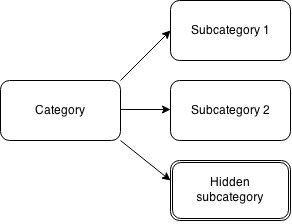
\includegraphics[width=\textwidth]{Chapters/Implementation/category-subcategories}
\caption{The structure where each category knows its subcategories}
\label{fig:catstructure}
\end{subfigure}
\begin{subfigure}[b]{0.4\textwidth}
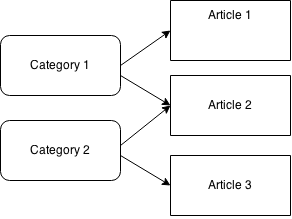
\includegraphics[width=\textwidth]{Chapters/Implementation/categories-articles}
\caption{The structure where each category know the title of its articles}
\label{fig:artstructure}
\end{subfigure}
\caption[The representation of the Wikipedia structure]{Combined this is the structure needed to represent the Wikipedia's underlying category structure as a graph}
\end{figure}


\subsubsection{Creating the Article graph}
It is also relevant to create a system of all the articles and their most describing categories, that is the categories shown at the bottom of the article page. The file containing all links between categories and their articles can be used to create a structure where each category knows its articles. Figure \ref{fig:artstructure}) illustrates this structure. 
\end{comment}
It is desirable to remove articles whose titles are not relevant for our project. Numbers without context is an example of Wikipedia article titles that are difficult to determine the meaning since a number could have various meanings, including temperatures, grades or years. Hence, all article titles which only contains numbers could be disregarded. Wikipedia contains many such articles, and a total of 23 227 articles where found. This reduces the number of links betweeen articles and categories as shown in table  \ref{tab:withoutnumber}.

\begin{table}[h]
\centering
\begin{tabular}{c|c}
\textbf{W/ Number Articles} & \textbf{W/o Number Articles}  \\ \hline
52 611 629 & 52 588 894
\end{tabular}
\caption[Number of links without number articles]{Number of links between categories and articles removed when articles only containing numbers are disregarded}
\label{tab:withoutnumber}
\end{table}


% 23227